% -----------------------------------------------
% Template for FA2025 Proceedings

% DO NOT MODIFY THE FOLLOWING SECTION!!
%-------------------------------------
\documentclass[11pt]{article}
\usepackage{fa2025}
\usepackage{amsmath}
\usepackage{cite}
\usepackage{url}
\usepackage{graphicx}
\usepackage{color}
\usepackage{siunitx}
\usepackage[utf8]{inputenc}
%-------------------------------------


\title{Comparing without classifying: evaluating embeddings from bioacoustic deep learning feature extractors}

\multauthor{
  Vincent S. Kather$^{1, 2*}$ 
  \hspace{1cm} 
  Burooj Ghani$^2$ 
  \hspace{1cm} 
  Dan Stowell$^{1, 2}$
  } { 
  $^1$ Department of Cognitive Science and Artificial Intelligence, Tilburg University, Netherlands\\
  $^2$ Naturalis Biodiversity Center, Leiden, Netherlands\\
% $^3$  Company, Address
  \correspondingauthor{vincent.kather@naturalis.nl}{Vincent S. Kather et al.}
}



\sloppy % please retain sloppy command for improved formatting
\begin{document}

%
\maketitle
\begin{abstract}
% In computational bioacoustics, deep learning models are composed of feature extractors and classifiers. 
% The feature extractors generate vector representations of the input sound segments, called embeddings. 
% The classifiers recognize a fixed number of classes most commonly representing different animal species. 
% Various benchmarks have been published to evaluate the classification performance. 
% While such benchmarking provides insight into specific performance statistics, it is limited to species that are included in the models training data. Furthermore, it makes it impossible to compare models trained on very different taxonomic groups. 
% This paper aims to address this gap by analyzing the generated embeddings of more than 15 bioacoustic models spanning a wide range of setups (model architectures, training data, training paradigms). 
% We investigate and evaluate different ways to quantify how models structure embedding spaces, which allows us to focus our comparison on feature extractors independent of classifiers. 
% We believe that this approach lets us evaluate the adaptability and generalization potential of models going beyond the classes they were trained on.
In computational bioacoustics, deep learning models are composed of feature extractors and classifiers. 
The feature extractors generate vector representations of the input sound segments, called embeddings. 
% The classifiers recognize a fixed number of classes most commonly representing different animal species. 
% Various benchmarks have been published to evaluate the classification performance. 
While benchmarking of classification scores provides insight into specific performance statistics, it is limited to species that are included in the models training data. Furthermore, it makes it impossible to compare models trained on very different taxonomic groups. 
This paper aims to address this gap by analyzing the embeddings generated by the feature extractor of more than 15 bioacoustic models spanning a wide range of setups (model architectures, training data, training paradigms). 
We evaluate and compare different ways how models structure embedding spaces through clustering and kNN classification, which allows us to focus our comparison on feature extractors independent of classifiers. 
We believe that this approach lets us evaluate the adaptability and generalization potential of models going beyond the classes they were trained on.
\end{abstract}

\keywords{\textit{
  deep learning, bioacoustics, embeddings
  }}
%

\section{Introduction}
\label{sec:introcution}

Human-driven climate change and deforestation have caused a rapid decline in global biodiversity \cite{gosselin_relationships_2018}.
Using sensor arrays for biodiversity monitoring, ecologists can gather information on environments and investigate how human pressures affect biodiversity and how we can halt its decline \cite{schmeller_building_2017}.
Passive acoustic monitoring (PAM) is one method that provides a low-cost and non-invasive way to monitor biodiversity \cite{sugai_terrestrial_2019}.
The vast amount of data generated by PAM sensors has led to the rapid development of bioacoustic deep learning models to help researchers reduce the annotation effort \cite{stowell_computational_2022}.
The use of these state-of-the-art models has proven valuable in ecological studies, for example in general species assessments \cite{cowans_improving_2024} or detection of endangered species \cite{allen-ankins_use_2025}.

While bioacoustic deep learning models are a useful asset in ecology, it is crucial to understand the model's limitations based on their training setup.
% little is known about how their training setup correlates to their performance.
The two main training strategies to develop bioacoustic deep learning models are supervised learning and self-supervised learning.
% In supervised learning large acoustic datasets are collected, annotated and used to train \cite{kahl_birdnet_2021}. 
Supervised learning models require large amounts of annotated data to be trained \cite{hagiwara_aves_2022}.
The models classify sounds based on a fixed number of predefined classes representing annotated sounds in the dataset.
While supervised learning can have the benefit of instructing models to differentiate between species vocalizations, it requires annotated datasets.
This limits supervised learning models to known and annotated classes and makes them sensitive to class imbalance and label quality.
% In self-supervised learning classes are defined by the model during training time \cite{baevski_efficient_2023,huang_masked_2022}.
Self-supervised learning can be executed in different ways.
In a paradigm referred to as masked prediction, the model is trained to predict a masked portion of the audio, thereby modelling bioacoustic characteristics without supervision \cite{huang_masked_2022}.
With growing annotated databases supervised learning models like Birdnet \cite{kahl_birdnet_2021} improve in performance, yet recent developments in self-supervised learning on models like Animal2vec \cite{schafer-zimmermann_animal2vec_2024} indicate a promising new direction for the field requiring less manual annotation.
Not requiring annotations, self-supervised learning models can be trained on far larger datasets, however there is no control of what is being learned.
The model might learn to differentiate between sounds based on very different characteristics than the species that produces them.

% The datasets that are created in this manner tend to feature many annotations for few classes and few annotations for many classes (long-tail distribution/class imbalance) \cite{arnaud_improving_2023}. 
% Models with a heavily imbalanced training dataset have shown to yield performance imbalances \cite{hamer_birb_2023}. 
% This implies that the models results are only reproducible when used to classify the well represented majority classes. 
% Furthermore, models trained in a supervised learning pipeline are restricted to only recognize a fixed set of classes. 
% Class imbalance and closed set recognition are two examples of phenomena, that show while supervised learning is the convention, it has shortcomings that restrict the usability of models trained in this way.

To evaluate bioacoustic deep learning models, a comparison of only the classifier performance obscures the fine-grained differences between models and how they analyze input sounds.
Bioacoustic deep learning models consist of artificial neural networks which can be subdivided into feature extractors and classifiers. 
The feature extractor creates an embedding (vector representation) of an input sound and the classifier (which corresponds to the final dense layer of the model) maps the embedding onto classes.
Commonly, in bioacoustics, a suite of established benchmarks is used to compare the classifier performance of state-of-the-art models \cite{hamer_birb_2023}.
This requires the models to have been trained on the classes present in the benchmarking datasets.
However, there is an alternative: using the embeddings created by the feature extractors, the generated embedding spaces can be analyzed in regard to their structural characteristics, irrespective of what the classifiers were trained on.

Output dimensions of feature extractors vary greatly, but it is uncertain if their dimensionality correlates to the downstream classifier performance. 
Dimensionality reduction algorithms are useful to standardize the dimensionality of different feature extractors, as well as help visualize the high dimensional embedding spaces.
% Due to the lack of separable clusters in ecoacoustics and soundscape analyzes, evaluation of embedding spaces (reduced to two dimensions) has become common in recent years \cite{sethi_characterizing_2020,calonge_revised_2024,parcerisas_categorizing_2023}. 
However, there is little investigation of how reducing the embedding space affects performance.
We therefore compare performance in both original and reduced embedding spaces.

Due to their size, datasets that are used to train bioacoustic models for bird detection are often based on citizen science data (e.g. xeno-canto \cite{xeno-canto_xeno-canto_2025}).
The majority of these recordings are focal recordings of individuals which are weakly labeled with little polyphony.
When models get applied to large PAM datasets, especially outside of North America (where the majority of the training data originates), the difference in recording conditions causes performance drops \cite{perez-granados_birdnet_2023}.
To accurately evaluate the models in this study, we use a PAM bird vocalization dataset from Colombia and Costa Rica \cite{vega-hidalgo_collection_2023}, as well as a dataset of frog vocalizations from Brazil \cite{canas_dataset_2023}.
Both datasets are comprised of PAM recordings in noisy environments and can therefore be considered as challenging datasets.
With this, we hope to on the one hand emphasize the performance differences between the models and on the other hand produce results that will reflect in real world applications.

This study aims to showcase the potential for evaluating and especially comparing bioacoustic deep learning models in regard to their training paradigm and training data.
This evaluation is based on the structuring capabilities of their respective feature extractors analyzed through clustering and classification performance.
Classification in this case refers to recognition of novel classes, as none of the models have been pretrained on the classes selected here.
This way single classification layers are attached to each feature extractor, all of which are trained on the same evaluation sets (bird and frog vocalizations), i.e. same classes and same data, allowing us to compare their performance.
Classification is done using a k-nearest neighbor (kNN) approach.
We perform our analysis in both the original embedding space and a reduced dimensional embedding space. 
That way we ensure the dimension is standardized for the second evaluation, whilst we can investigate performance differences between the original embedding space and the reduced space.
% This study will therefore examine how different dimensionality reduction strategies impact performance. 
% While the possibilities of analysis of these high dimensional embedding spaces are vast, we limit ourselves to 
% Performance will be evaluated through an analysis of clustering based on
% \begin{enumerate}
%     \item Silhouette Score \cite{rousseeuw_silhouettes_1987}, 
%     \item Adjusted Rand Index \cite{steinley_variance_2016} based on KMeans clustering and
%     \item Adjusted Mutual Information \cite{romano_standardized_2014} based on KMeans clustering.
% \end{enumerate}
% To do so, we analyse clusterings of deep learning feature extractors and use them to compare different training setups.
This method of analysis opens up the possibilities for a fair comparison of deep learning feature extractors guiding the field to a better understanding how training configurations affect downstream performance.
% Summary of what we are contributing.






\section{Methods}
\label{sec:methods}


\begin{table*}[t]
  
  \caption{List of feature extractors compared in this study. Columns "abbrev." shows the an abbreviated name used in Figures \ref{fig:subl_vs_ssl} and \ref{fig:orig_vs_ump}. "training" shows the training setup chosen during training, i.e. ssl for self-supervised learning, sup l for supervised learning and ft for fine-tuning. The "architecture" column more specifically describes the model architecture used. "dimension" shows the output dimension of the feature extractor. "trained on" summarizes the species group that was used to train the model. "ref." provides the respective publication for a given model. }
  \label{tab:bacpipe_models}
  \centering
  \begin{tabular}{|l|c|c|c|c|l|c|}
    \hline
    name& abbrev. & 
    training & architecture &
    dimension & trained on & ref.\\
      %  ref paper&
      %  ref code&
      %  sampling rate&
    \hline
    Animal2vec\_XC      & brdnet   & ssl & d2v2.0 & 768 & birds & \cite{schafer-zimmermann_animal2vec_2024}\\
    Animal2vec\_MK      & a2v\_xc  & ssl + ft & d2v2.0 & 1024& meerkats & \cite{schafer-zimmermann_animal2vec_2024}\\
    AudioMAE            & a2v\_mk  & ssl + ft & ViT 	 & 768 & general & \cite{huang_masked_2022}\\
    AVES\_ESpecies      & aud\_mae   & ssl + ft & HuBERT 	 & 768 & general + animals & \cite{hagiwara_aves_2022}\\
    AvesEcho\_PaSST     & aves   & sup l & PaSST 	 & 768 & birds & \cite{ghani_generalization_2024}\\
    BioLingual          & bioling  & mm sup l & CLAP 	 & 512 & animals + birds & \cite{robinson_transferable_2023}\\
    BirdAVES\_ESpecies  & birdaves   & ssl + ft & HuBERT 	 & 1024& general + birds & \cite{hagiwara_aves_2022}\\
    BirdNET             & aecho   & sup l & EffNetB0 	 & 1024& birds & \cite{kahl_birdnet_2021}\\
    % HumpbackNET         & 3.9 & sup l & ResNet50 	 & 2048& hb whales& \cite{kather_development_2024}\\
    Google\_Whale       & i66   & sup l & EffNetB0 	 & 1280& whales & - \\
    Insect459NET        & i459 & sup l & EffNetv2s 	 & 1280& insects & - \\
    Insect66NET         & perch & sup l & EffNetv2s 	 & 1280& insects & - \\
    % Mix2                & 3   & sup l & MobNetv3 	 & 960 & frogs & \cite{moummad_mixture_2024}\\
    NonBioAVES\_ESpecies & p\_clr    & ssl + ft & HuBERT 	 & 1024& general + non-bio & \cite{hagiwara_aves_2022}\\
    Perch\_Bird         & s\_perch   & sup l & EffNetB0 	 & 1280& birds & - \\
    ProtoCLR            & g\_whale   & sup l 	 & CvT-13 & 384 & birds & \cite{moummad_domain-invariant_2024}\\
    % RCL\_FS\_BSED       & 0.2 & sup cl 	 & ResNet9 	 & 2048& dcase task 5 & \cite{moummad_regularized_2024}\\
    SurfPerch           & nonbioaves   & sup l & EffNetB0 	 & 1280& coral reefs + birds & \cite{williams_leveraging_2024}\\
    % VGGish              & 0.96& sup l & VGG & 128 & general & \cite{hershey_cnn_2017}\\
    \hline
  \end{tabular}
\end{table*}


To incorporate a variety of training setups, covering popular models as well as models targeted to various species groups, we compare a total of 15 pretrained bioacoustic feature extractors (Table \ref{tab:bacpipe_models}).
This includes both self-supervised and supervised learning feature extractors. 
Furthermore, large variations in input length, embedding dimension and training data provide a diverse landscape of feature extractors, allowing us to analyze performance of differently structured embedding spaces.

\subsection{Dataset}
\label{ssub:dataset}

The evaluation datasets that were used for this study are a bird vocalization dataset (bird dataset) recorded in coffee farms in Colombia and Costa Rica \cite{vega-hidalgo_collection_2023} and a frog vocalization dataset (frog dataset) recorded in Brazil \cite{canas_dataset_2023}.
The recordings in these datasets feature challenging soundscape recordings with overlapping vocalizers and noisy environments.
Both datasets have been reduced from their original size to only include sound events corresponding to classes with more than 150 annotations.
Due to the high amount of polyphony, the frog dataset has furthermore been reduced to only contain sound events with non-overlapping annotations, i.e. turning it into a single-label dataset.
It is worth mentioning, that by excluding overlapping annotations, only polyphony of frog species is removed, the complex background of overlapping sounds created by insects and birds in the recordings remain.

For the bird dataset this results in 11 classes, while for the frog dataset 18 classes are included in the final dataset.
We intentionally selected soundscape recordings with gradual changes of background noise and overlapping species vocalizations to amplify the differences between the feature extractors' capabilities to structure the data.




\subsection{Data pipeline}
\label{ssub:data_pipe}

For each of the feature extractors, the respective model code base was cloned, and the model was stripped of its classifier.
For both animal2vec feature extractors, outputs from the attention heads and input lengths are averaged, resulting in one embedding per input segment (as is the case with all other feature extractors).
Data are imported from the sound files, resampled to the model-specific sample rate, and padded to fit the model-specific input length.
All the necessary code to reproduce the computations can be found in the repository \textbf{bacpipe}\footnote{\url{github.com/bioacoustic-ai/bacpipe}} (\textbf{b}io\textbf{a}coustic \textbf{c}ollection \textbf{pipe}line).

\subsection{Methods for evaluating embedding spaces}
\label{ssub:eval_dim_reduc}

Embedding spaces are evaluated using clustering and classification.
Our primary focus is the comparison of the two paradigms: supervised learning and self-supervised learning.
Furthermore, we explore how the data chosen for training affects the clustering capabilities of different feature extractors.


% Given the high dimensional nature of embedding spaces, any quantitative evaluation may be subject to the curse of dimensionality \cite{bellman_dynamic_1957}.
% This refers to the issues that arise when dealing with comparatively small number of datapoints in very high dimensional space.
% In our setup this is relevant as the dimensions vary greatly and any resulting distance based calculations will be affected differently if they are calculated spaces of varying dimensions. 
% Therefore, we aim to evaluate in what way reducing the dimension of embedding spaces impacts performance for each of the feature extractors.
% The underlying assumption is that by homogenizing the dimension of the very differently structured embedding spaces, we lay the groundwork for quantitatively comparing the different feature extractors.

% % Therefore, we must first assess how reducing the dimension affects the performance of each feature extractor.
% Initially, feature extractor performance will be analysed using clustering performance and subsequently the performance of the reduced embedding spaces will be compared in the same way and related back to the initial performance values.
% We will compare two versions of linear dimensionality reduction algorithms, principal component analysis (PCA) \cite{wold_principal_1987} and sparse principal component analysis (sPCA) \cite{zou_sparse_2006} as well as one non-linear dimensionality reduction algorithm, uniform manifold approximation projection (UMAP) \cite{mcinnes_umap_2020}.
% Clustering performance will be analysed using Silhouette Score (SS) \cite{rousseeuw_silhouettes_1987}, Adjusted Rand Index (AIR) \cite{steinley_variance_2016} and Adjusted Mutual Information (AMI) \cite{romano_standardized_2014}.

% Reducing dimensions using linear transformations has the advantage of preserving relative distances between all data points.
% This means that quantitative analyses involving distance based calculations can be performed in the lower dimensional space.
% Non-linear dimensionality reduction like UMAP however, creates a learned transformation based on a graph structure of the data and therefore disregards distances between data points \cite{mcinnes_umap_2020}.
% While it is claimed that UMAP preserves relative distances for within cluster points, transformed relative distances between clusters are not representative of distances in the original high dimensional space.

% To evaluate the changing embedding spaces as a function of the dimensionality reduction method, clustering performance will be evaluated. Adjusted Rand Index (AIR) \cite{steinley_variance_2016} and  
The clustering is computed using KMeans with the same number of clusters as classes in the ground truth. 
Clustering performance is evaluated using Adjusted Mutual Information (AMI) \cite{romano_standardized_2014} to compare the KMeans clustering with the ground truth.
% Adjusted Rand Index is not included in this study, as it focuses on how well data points are grouped in a clustering, whereas we are primarily interested how well the KMeans clustering agrees with the ground truth labels.
% Non-linear dimensionality reduction algorithms like UMAP create a learned transformation based on a graph structure of the data and therefore disregards distances between data points \cite{mcinnes_umap_2020}.
% Silhouette Score is also not included in this comparison as the challenging dataset yielded very low performance and variance, making a meaningful comparison impossible.
% AMI and ARI require a clustering to be computed, to then quantify the agreement between that clustering and the ground truth and are therefore applicable to non-linear dimensionality reductions.
% AMI measures how well clusters share information while ARI quantifies how well points are grouped.

Performance is also evaluated by training a simple kNN classifier on each of the embedding spaces with a nearest neighbor parameter of 15.
% The linear classifier is trained on the 11 and 18 classes for the bird and frog datasets respectively for 10 epochs with a batch size of 64 and a learning rate of 0.001. 
% For the kNN classifier a nearest neighbor parameter of 15 is chosen.
The classifier is trained on the 11 and 18 classes for the bird and frog datasets respectively.
Data is split into train, validation and test set in the ratio 0.65:0.15:0.2.
Performance is evaluated using a balanced macro accuracy score \cite{brodersen_balanced_2010} to handle the imbalance in class sizes.

Evaluations are computed in both the original embedding spaces and an embedding space reduced to 300 dimensions.
This way the embedding dimension is standardized and performance can be compared while controlling for this factor.
% It also allows us to compare the performance of each model in their high dimensional original embedding space, as well as in a reduced dimension.
% For the linear classifier, to preserve relative distances between data points, Principal Component Analysis (PCA), a linear dimensionality reduction is selected.
Uniform manifold approximation projection (UMAP) \cite{mcinnes_umap_2020} is selected for the dimensionality reduction to 300 dimensions.
UMAP is also used to visualize the embeddings in two dimensions in Fig. \ref{fig:embeds}.

\section{Results}
\label{sec:results}

\begin{figure*}[ht]
    \centerline{\framebox{
    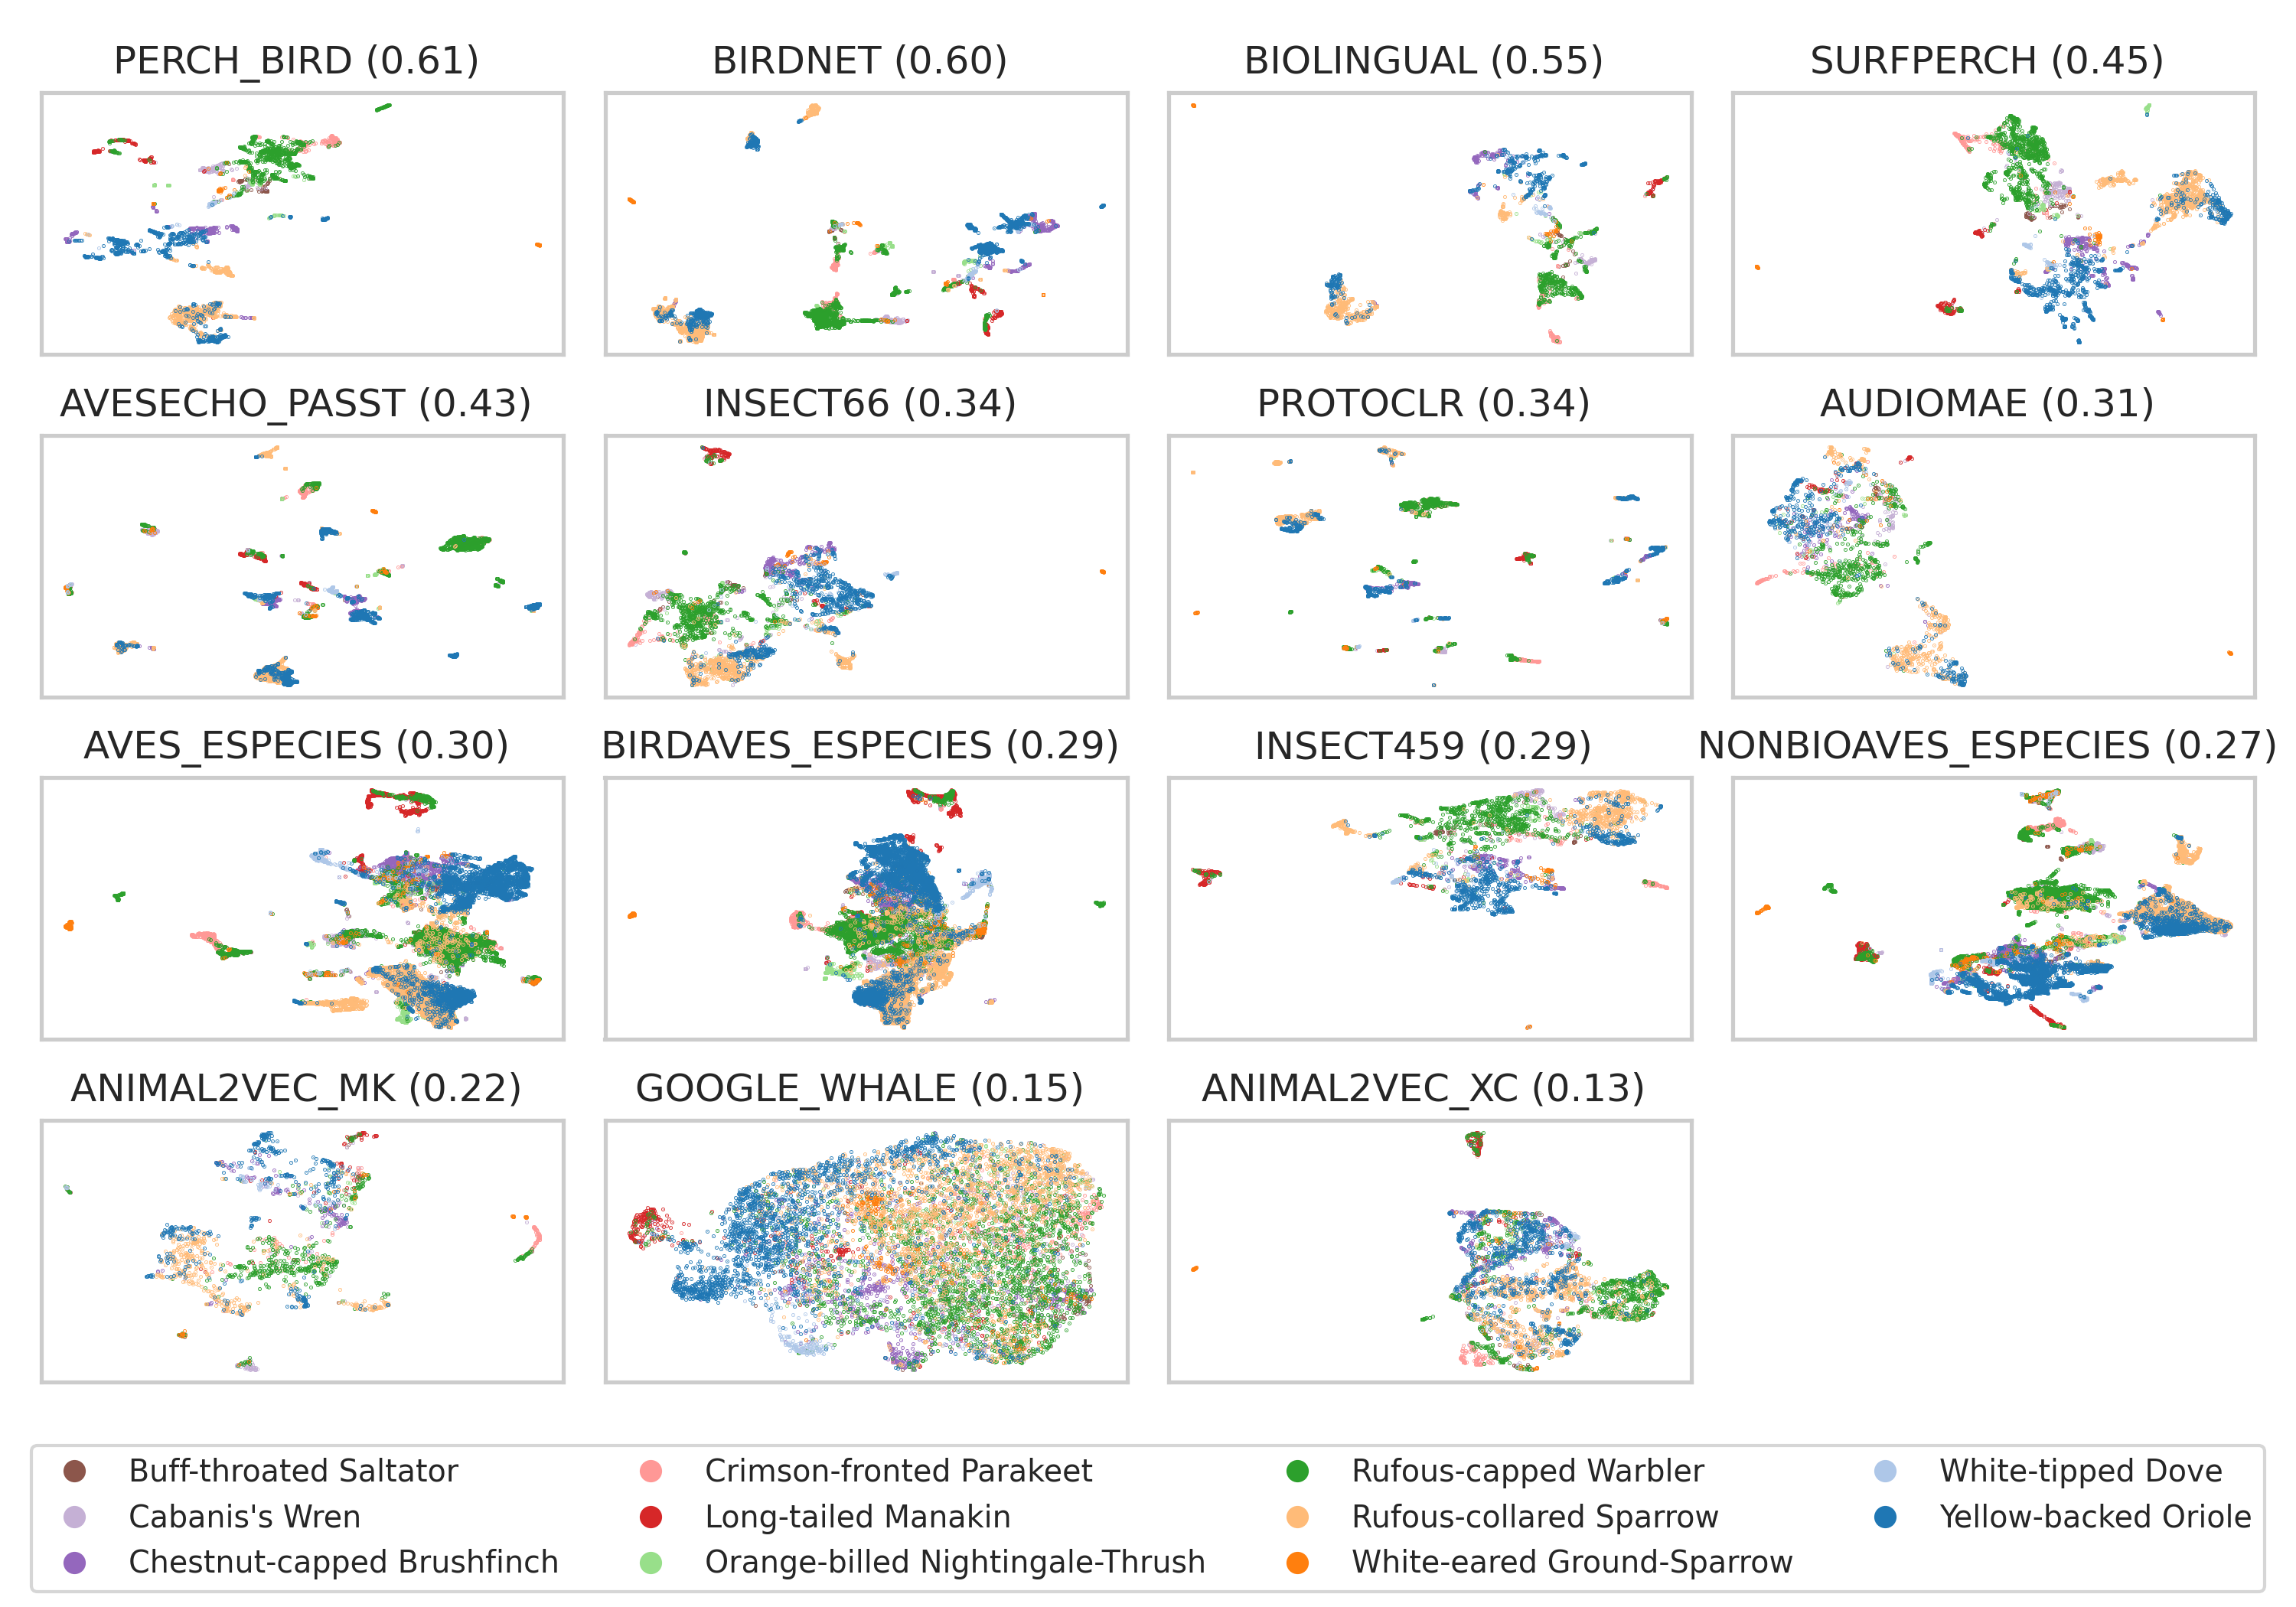
\includegraphics[width=16.3cm]{Sections/imgs/normal_overview.png}}}
    \caption{Two-dimensional embedding spaces of all feature extractors, sorted descending by their clustering performance of AMI values (indicated next to their name) from top left to bottom right.
    % Given the different input lengths of the feature extractors, the number of embeddings vary significantly.
    Colors correspond to the class labels, which are 11 different tropical bird species.}
    \label{fig:embeds}
\end{figure*}

% Embeddings spaces of are visualized using UMAP in are generated from the input data using all feature extractors and then the dimensionality reduction algorithm UMAP is used to visualize the data in two dimensions.
% The results are shown in Fig. \ref{fig:embeds}.

Two-dimensional UMAP embeddings are shown in Fig.~\ref{fig:embeds}.
The worst performing feature extractors, produce large unstructured clouds of mixed color, indicating that no significant clustering is achieved.
In the first and second row, feature extractors can be seen to separate the embeddings into meaningful clusters.
It is noticeable that some feature extractors such as AvesEcho\_PaSST and ProtoCLR seem to generate more subclusters than most other feature extractors.
The seven best performing feature extractors are all trained using supervised learning and the top three additionally trained on bird vocalizations.
All three of the AVES models (BirdAVES, AVES and NonBioAVES) reach similar performances in spite of big differences in their fine-tuning datasets \cite{hagiwara_aves_2022}.


\begin{figure}[ht]
    \centerline{\framebox{
    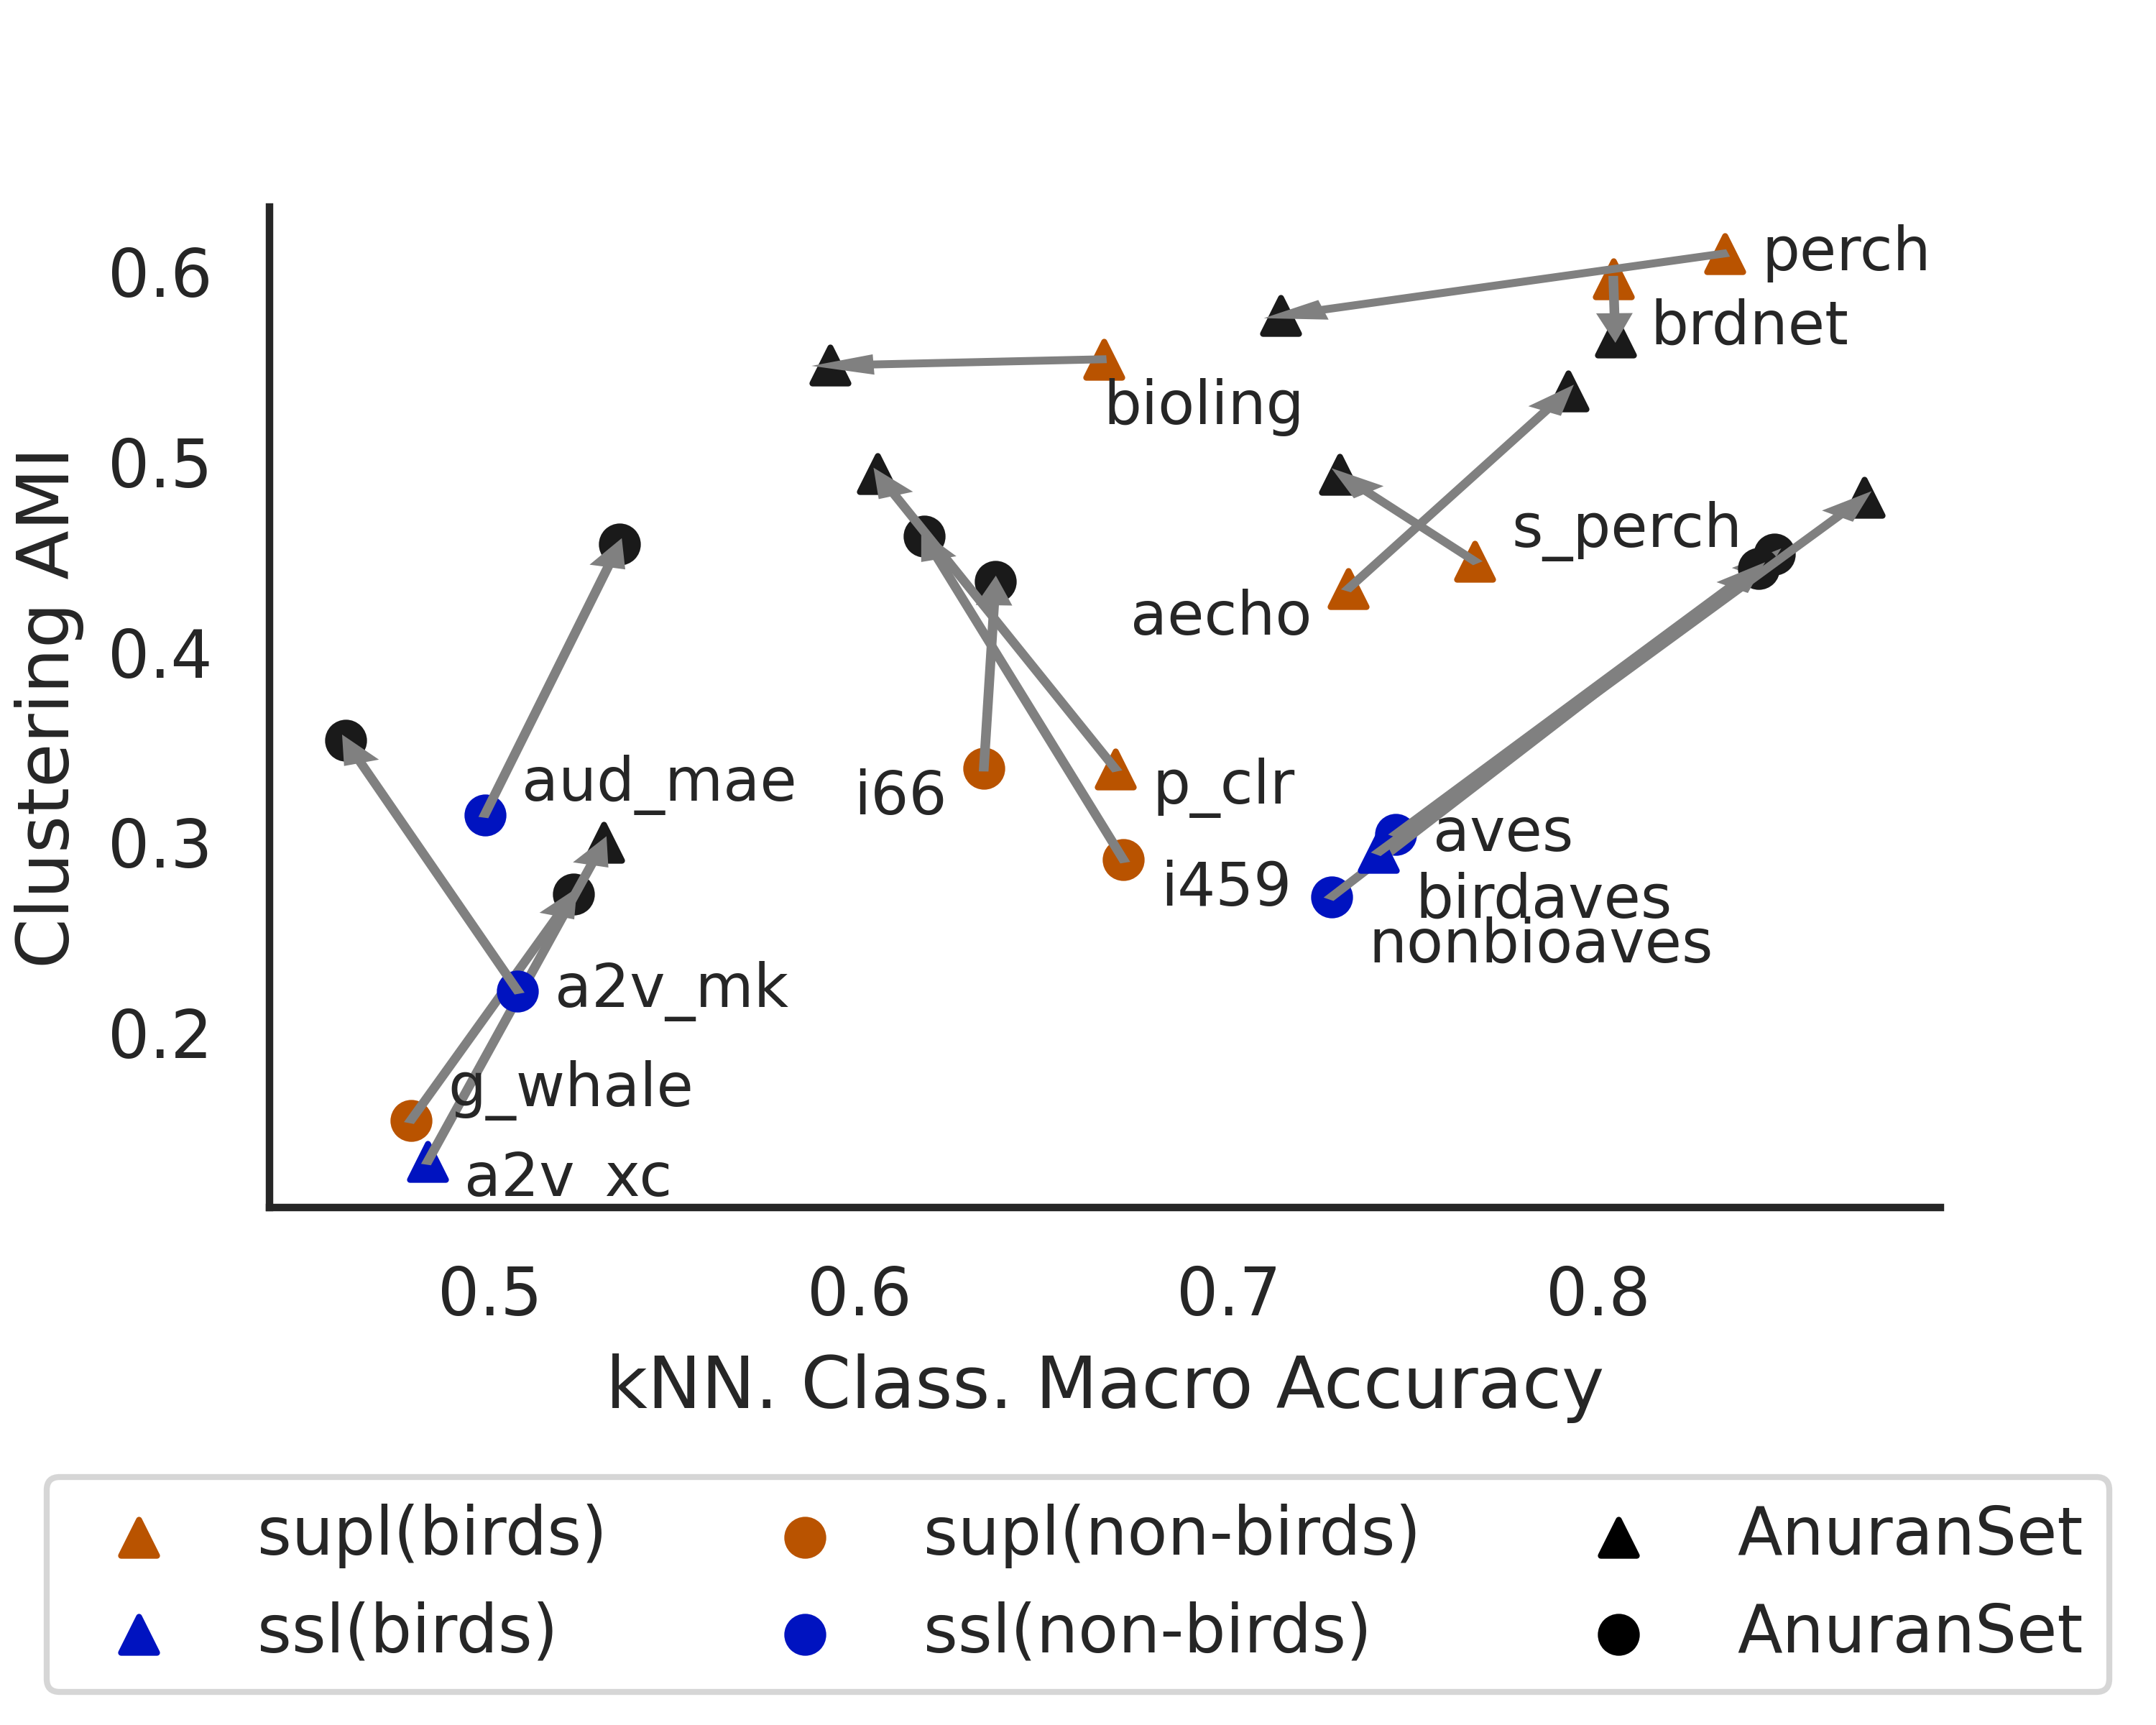
\includegraphics[width=7.8cm]{Sections/imgs/scatterplot_clust_vs_class_neotrop_anuran_normal.png}}}
    \caption{Comparison of feature extractor performance by learning paradigm, training data and application data. 
    Abbreviated names correspond to abbrev. column in Tab.~\ref{tab:bacpipe_models}. 
    The x-axis shows clustering results of AMI while the y-axis shows macro accuracy results of kNN classification. 
    Colors correspond to supervised learning and self-supervised learning feature extractors, while symbols separate bird and non-bird training data.
    Black points show the performance of each feature extractor on the frog dataset.
    Red and blue points show the performance on the bird dataset. 
    The gray arrow shows the performance change from the bird to the frog dataset.}
    \label{fig:orig_vs_ump}
\end{figure}
    

To highlight performance changes once the feature extractors are applied to a dataset different from their training domain, Fig. \ref{fig:orig_vs_ump} shows the performance on the bird dataset (black) and the frog dataset (red and blue) connected by an arrow.
Performance is evaluated by macro accuracy of knn classification on the x-axis and AMI of clustering on the y-axis.

First we will focus on the feature extractors being applied to the bird dataset, shown in red and blue.
When focussing on the y-axis, all self-supervised learning feature extractors (in red) reach clustering performances under 0.31 while the 6 best performing feature extractors are trained using supervised learning.
Performance by kNN classification is more equally distributed, however, again supervised learning feature extractors reach the three highest values.
Furthermore, Animal2vec\_XC, the only self-supervised learning feature extractor that was not fine-tuned, performs poorly by both clustering and kNN classification.
Google\_Whale represents the only supervised learning feature extractor performing very poorly by clustering and kNN classification.

Comparing by training data, feature extractors trained on only or including bird datasets outperform the other feature extractors by kNN classification and even more so by clustering.
Aside from ProtoCLR the supervised learning models that are also trained on birds vastly outperform all other models in the combination of clustering and kNN classification.
Perch and BirdNET lead in both clustering and kNN classification by a large margin.
Biolingual, which was trained on large bird databases using a multi-modal approach performs well by clustering, but comparatively poorly by kNN classification.

The arrows show the performance change when the feature extractors are applied to the frog dataset.
All self-supervised feature extractors improve in clustering performance and aside from Animal2vec\_MK also in kNN classification.
The self-supervised AVES feature extractors (BirdAVES, AVES and NonBioAVES) drastically improve in both clustering and kNN classification on the frog dataset.
So much so, that all three outperform all other feature extractors by kNN classification.
% Aside from all feature extractors increase in clustering performance.
Among supervised learning feature extractors, changes in both clustering and kNN classification performance are more varied.
Especially the three best performing models by clustering for the bird dataset, Perch, BirdNET and Biolingual, all decrease in performance when applied to the frog dataset.

All non-bird trained feature extractors improve in clustering.
From the supervised bird trained feature extractors, only AvesEcho improves in both clustering and kNN classification.
Again, when applied to the frog dataset, all bird trained feature extractors except for Animal2vec\_XC outperform the rest by clustering.
The top 6 models by clustering are again the supervised learning bird trained feature extractors.
However, by kNN classification, results are more mixed by both training paradigm and training domain.

When referring back to Table \ref{tab:bacpipe_models} embedding dimension does not correlate with clustering or kNN classification performance.
Furthermore, the only two feature extractors trained on marine sounds, Google\_Whale and SurfPerch (trained on birds and marine sounds) reach very different performances.
    


\begin{table}[t]
  
  \caption{List of feature extractors compared in this study. }
  \label{tab:results}
  \centering
  \begin{tabular}{|l|ccc|}
    \hline
    \textbf{bird data}& \multicolumn{3}{c|}{classification (macro accuracy)} \\
    \hline
    category &
    original &
    umap &
    pca \\
    \hline
    ssl & 0.617& 0.619& 0.587 \\
    supl & 0.695& 0.711& 0.66 \\
    bird & 0.712& 0.723& 0.607 \\
    non-bird & 0.609& 0.618& 0.658 \\
    \hline
    & \multicolumn{3}{c|}{clustering (AMI)} \\
    \hline
    ssl & 0.256& 0.405& 0.25 \\
    supl & 0.418& 0.476& 0.414 \\
    bird & 0.426& 0.479& 0.411 \\
    non-bird & 0.271& 0.413& 0.276 \\
    \hline
    \textbf{frog data}& \multicolumn{3}{c|}{classification (macro accuracy)} \\
    \hline
    category &
    original &
    umap &
    pca \\
    \hline
    ssl & 0.682& 0.679& 0.601 \\
    supl & 0.668& 0.655& 0.673 \\
    bird & 0.705& 0.698& 0.629 \\
    non-bird & 0.638& 0.627& 0.662 \\
    \hline
    & \multicolumn{3}{c|}{clustering (AMI)} \\
    \hline
    ssl & 0.414& 0.508& 0.418 \\
    supl & 0.488& 0.546& 0.49 \\
    bird & 0.5& 0.558& 0.503 \\
    non-bird & 0.411& 0.5& 0.414 \\
    \hline
  \end{tabular}
\end{table}


% ssl & 0.617& 0.619& 0.587 \\
% supl & 0.695& 0.711& 0.66 \\
% bird & 0.712& 0.723& 0.607 \\
% non-bird & 0.609& 0.618& 0.658 \\
% \\hline
    
% \\hline
% ssl & 0.256& 0.405& 0.25 \\
% supl & 0.418& 0.476& 0.414 \\
% bird & 0.426& 0.479& 0.411 \\
% non-bird & 0.271& 0.413& 0.276 \\
% \\hline
    
% \\hline
% category &
% original &
% umap &
% pca \\
% \\hline
% ssl & 0.682& 0.679& 0.601 \\
% supl & 0.668& 0.655& 0.673 \\
% bird & 0.705& 0.698& 0.629 \\
% non-bird & 0.638& 0.627& 0.662 \\
% \\hline
    
% \\hline
% ssl & 0.414& 0.508& 0.418 \\
% supl & 0.488& 0.546& 0.49 \\
% bird & 0.5& 0.558& 0.503 \\
% non-bird & 0.411& 0.5& 0.414 \\


Table \ref{tab:results} shows the averaged performances over all feature extractors in the different categories: supervised and self-supervised learning and bird and non-bird.
Firstly we want to point out the performance changes following dimensionality reduction using UMAP.
For evaluation with both bird and frog datasets, UMAP embeddings improve the clustering results significantly for every category.
For the classification performance values are very similar between original and UMAP reduced embeddings, however, while for the bird dataset UMAP yields to performance increases for most categories, for the frog dataset, the original embeddings yield better restults.
In line with Fig. \ref{fig:orig_vs_ump}, supervised learning outperform the self-supervised learning feature extractors by a large margin for classification and clustering in the bird dataset.
For the frog dataset, due the the improved performance of the AVES models, self-supervision outperforms supervised learning by kNN classification.
When comparing the values between all categories, the bird trained feature extractors outperform all other categories for both evaluation sets.


\section{Discussion}
\label{sec:discussion}

Although the self-supervised feature extractors represented in this study are trained on very large datasets, their combined performance is inferior to most of the supervised learning feature extractors including those trained on non-bird categories.
Perch and BirdNET \cite{kahl_birdnet_2021}, both of which are trained on thousands of classes of bird vocalizations vastly outperform the other feature extractors. 
It is worth mentioning that they do so, while being trained on standard EfiicienNETs.
Similarly, SurfPerch \cite{williams_leveraging_2024} and AvesEcho\_PaSST \cite{ghani_generalization_2024}, both of which have largely benefited from Perch or BirdNET pretraining, perform well by both clustering and classification.
More generally, the embedding spaces of feature extractors trained on very large annotated bird song datasets seem to yield good separation between clusters.

% Interestingly, Insetct66 and Insect459 both of which were trained on only insect sounds and far fewer classes than the bird-trained biolingual, vastly outperform it in classification.
As stated in the introduction, self-supervised learning models lack supervision and might therefore learn classes not meaningful to differentiate between species vocalizations.
When comparing Figures \ref{fig:embeds} and \ref{fig:orig_vs_ump} we observe poor clustering both in terms of AMI performance and by qualitative visual analysis of the embedding separation, which could be resulting from non-meaningful classes.
However, for the three AVES feature extractors, the classifier is nontheless able to learn a meaningful differentiation between the classes.
This could be attributed to the fact, that while they are self-supervised, the training data consisted of curated and non-sparse sound events, thereby increasing the likelihood that meaningful classes are learned.
The drastic performance increase of all three AVES models when evaluated with the frog dataset highlights that in this case the self-supervision enabled the extraction of meaningful features despite the domain shift.

For the self-supervised learning feature extractors, fine-tuning seems to only marginally improve performance.
The three feature extractors based on the AVES models all share the same general audio pretraining and architecture but differ largely in fine-tuning. 
The similarity in performance indicates that the dominant influence on the structuring of embeddings is defined by either the pretraining or the architecture.
Animal2vec\_XC and Animal2vec\_MK, the latter of which is fine-tuned, largely share the same architecture but were trained on very different datasets.
Yet, both models reach similarly bad performance, this is especially surprising for the fine-tuned Animal2vec\_MK.
For the supervised learning feature extractor SurfPerch, which was developed for marine data in coral reefs, bird training data from Perch was mixed with coral reef sounds during pretraining.
While the target domain is very different from the bird dataset, SurfPerch still reaches very high performance.
This performance drops in terms of classification though, as soon as the target domain is shifted to the frog dataset.
Again, this indicates that including data of the target domain is more effective during pretraining than fine-tuning.

While the dimensions of the feature extractors vary greatly, performance does not correlate with dimension.
Nonetheless, in Tab. \ref{tab:results} we demonstrated that using a standardized embedding space affects clustering and classification performance differently.
The performance differences that can be observed are predominantly in clustering, indicating that the graph structure, which KMeans builds for the clustering, is aided by dimensionality reduction using UMAP.
For this study dimensionality reduction using Principal Component Analysis was also performed and evaluated using linear classification, however, performance only changed marginally and was therefore omitted from this comparison.

This analysis underlines the high quality of embeddings created by large supervised learning feature extractors like BirdNET and Perch.
While their training domain aligned with the domain bird dataset, so did that of biolingual, Animal2vec\_XC and BirdAVES\_ESpecies, none of which reached performance metrics similar to BirdNET and Perch.
The dramatic decrease in classification performance by Perch raises the question if the fact that Perch's training data is comprised of solely xeno-canto recordings makes it less domain agnostic than BirdNET which was trained on selected curated bird datasets along with a large portion of xeno-canto.

This study is meant to present a workflow for a more in-depth analysis of embedding spaces, which can be reproduced with the provided repository bacpipe\footnote{\url{github.com/bioacoustic-ai/bacpipe}}.
Evaluation through clustering and classification has shown to vary significantly when applied to the different evaluation sets, undermining the use of both metrics to better understand how training setup affects performance.
By establishing a default analyses of feature extractors alongside the common classification benchmarks, bioacoustic research can accelerate towards a better understanding of what training characteristics are beneficial in this domain.

\section{Conclusion}
\label{sec:conslusion}

In this study we have compared a variety of different state-of-the-art bioacoustic deep learning models, representing different training paradigms and training domains.
To compare the models, we have isolated their feature extractors and used them to generate embeddings of a curated evaluation dataset consisting of annotated bird and frog sounds.
The aim of this study was to firstly present a large comparison of very different bioacoustic deep learning feature extractors and to evaluate how training paradigms and training domains affect performance.
Performance was evaluated through clustering using an AMI score and through kNN classification using a macro accuracy score.

We have shown that in spite of recent improvements, bioacoustic feature extractors still struggle with polyphonic PAM datasets, especially if they are outside of the training domain.
At this point, self-supervised learning performance is still inferior to that of supervised learning models.
This performance difference is visible in both kNN classification and even more in clustering.
Furthermore, we have shown that alignment of training domain and target domain during pretraining impacts performance more, than during fine-tuning.
This study presents a roadmap for a more in-depth performance evaluation of bioacoustic deep learning models, allowing for a better understanding of how training setup impacts downstream performance.



\section{Acknowledgments}
A lot of work went into developing each of the feature extractors presented here, and we highly appreciate that they are made publicly available.
We would also like to acknowledge Álvaro Vega-Hidalgo and his coauthors, who collected, assembled and annotated the dataset used to evaluate the feature extractors. 
This project is funded by the Marie Skłodowska-Curie doctoral network BioAcousticAI.
% For bibtex users:
% \bibliography{FA2025_template}
\bibliography{References}


\end{document}
